%%==========================
%% chapter01.tex for SJTU Master Thesis
%% based on CASthesis
%% modified by wei.jianwen@gmail.com
%% version: 0.3a
%% Encoding: UTF-8
%% last update: Dec 5th, 2010
%%==================================================

%\bibliographystyle{sjtu2} %[此处用于每章都生产参考文献]
\chapter{绪论}
\label{chap:what}

\section{研究背景}

%\begin{figure}[!htp]
  %\centering
  %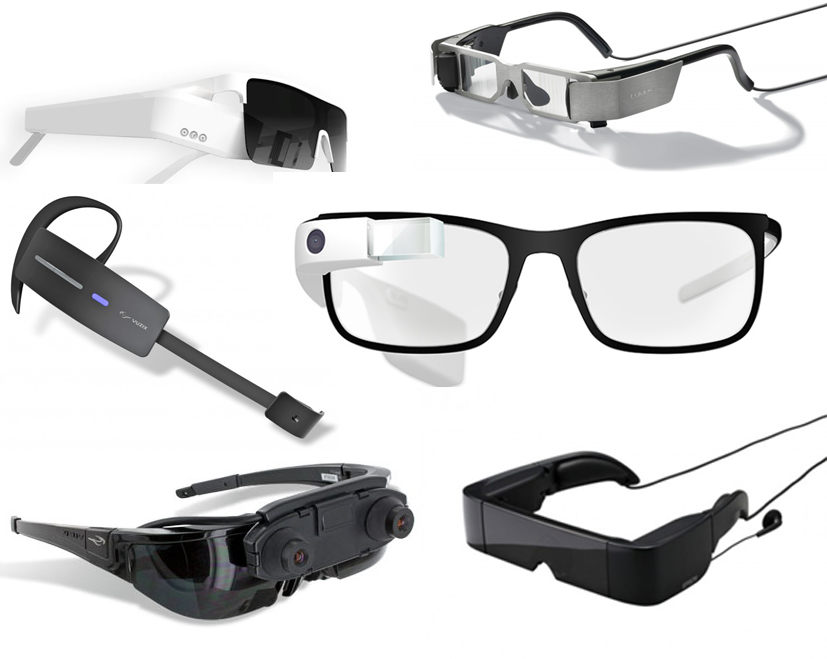
\includegraphics[width=0.8\textwidth]{chap1/ARGlasses}
  %\bicaption[fig:glasses]{增强现实设备}{增强现实设备}{Fig.}{Augmented Reality devices}
%\end{figure}

增强现实(Augmented Reality)是一种将虚拟场景融合进真实场景的技术,其中包括虚拟物体与现实的结合、即时互动以及三维的特性。
增强现实技术可以提供现实中无法获取的信息,用户通过附加的虚拟信息提升对现实场景的了解,增强现实技术在医疗、工业、娱乐与教育上都有广泛的应用前景。
Azuma等人在1997年和2001年\upcite{azuma1997survey,azuma2001recent}及Feng Zhou等人\upcite{FengZhou:2008:TAR:1605298.1605333}在2008年综述了增强现实所需的环境设置、追踪技术、交互技术、用户界面、显示技术及应用发展趋势。

而混合现实(Mixed Reality)则是介于虚拟场景和真实场景之间的一种形态,从图\ref{fig:mr}中看到Milgram\upcite{Milgram:2009:TDC:1643928.1643932}对混合现实,虚拟现实以及真实场景的渐变过程划分,混合现实包含了增强现实与虚拟现实。

\begin{figure}[!htp]
  \centering
  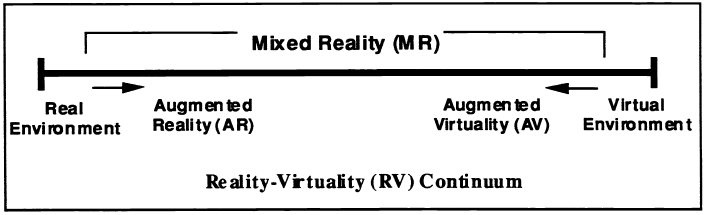
\includegraphics[width=0.95\textwidth]{chap1/Milgram_Continuum}
  \bicaption[fig:mr]{混合现实}{混合现实\upcite{milgram1995augmented}}{Fig.}{Mixed Reality\upcite{milgram1995augmented}}
\end{figure}

随着Google Glass\upcite{googleglass}的上市,智能眼镜成了2014年增强现实与混合现实领域最期待的设备之一。
%,从图\ref{fig:glasses}可见现在炙手可热的一批增强现实穿戴式设备。
眼镜最大的特征在于不需要用户手持进行操作,这一点诸如手机、平板或者更为累赘的台式机、笔记本是完全无法比拟的。
并且眼镜的视野十分宽阔,基本可以覆盖人眼的整个视野,虽然现在的手机越做越大,平板的普及性也很高,但是用户依然可以感受到这些智能设备的边界,而眼镜,就没有这样的局限性。
因而针对眼镜此类设备的研究及其与增强和混合现实应用的结合正是近些年来的研究热点。

针对不一样的设备,关于多点触控、手势、语音控制等多种交互通道的研究层出不穷。
一种类型的交互系统使用单一的通道进行交互,比如平板电脑上的多点触控,或者使用摄像头进行手势识别,再有些利用遥感等传感器进行不同指令的发送。
考虑到视觉通常会受到外界不相干信息干扰,语音控制也是非常直观的一种方式。
另一种类型的交互系统则综合多种通道协作进行交互,诸如利用压力传感,电流反馈等释放双眼、双手的交互方式。
%尽管手势交互因其直观在交互手段中占据了大部分应用,但多种交互手段的尝试对本文的研究是很有必要的。

除了交互手段对增强和混合现实应用有着举足轻重的影响以外,如何在不同的状态间切换、如何区分不同的状态,虽然是一个应用细节,却也极大地影响用户的使用体验。
同样的情形如果在桌面应用上,可能就是一个鼠标点击的区别,即便是最糟糕的情况也莫过于切换过于频繁,让用户很难继续之前的任务。

但在增强现实和混合现实的应用环境下,整个工作环境与输入空间都不是严格固定的,诸如最基本的拖拽还是单纯的移动都无法直接识别,需要通过其他的辅助或者设定才可以完成,因而对于不同交互手段如何在状态间切换也是一个研究热点。
目前状态切换存在着容易混淆\upcite{TrackingBased}、呈现不自然\upcite{Selection}及增加记忆负担\upcite{SideBySide}等问题,值得进一步研究。

与此同时,在对增强和混合现实应用的调研中发现,多数应用都涵盖模型的使用,而关于这点通常都以导入模型来处理。
导入模型虽然简单易行但受控于应用自身的数据库,而且用户无法根据自己的想法创建自定义的符合当前场景的模型。
针对三维建模这一应用场景,现下已经有很多相关的轻量级软件,可以通过简单的操作构建出复杂又美观的模型来。
但在增强和混合现实的应用条件下,哪些设计可以保留并提升,哪些需要舍弃则是另一个需要进一步探索的研究点。
因而需要对物体创建应用在不同的平台如桌面应用、手持移动设备和释放双手的穿戴设备做调研。

桌面应用普遍基于单击工具完成,如Google Sketch\upcite{sketchup}和TinkerCAD\upcite{tinkercad},对于工具的设计是一个很好的切入点。
而其他手持设备在基于单手操作的限定条件下对建模应用进行的设计就非常值得借鉴,比如指尖绘制,通过自制的标签笔进行绘制等,还有释放双手的场景中结合三维场景和平板同时进行模型设计的方法。
其中对于用户建模的难点主要集中在(1)如何克服用户自身不同的绘制水平,帮助用户改善自己的模型。(2)如何提供用户足够的自由度创建有自己特色的模型,不受限于应用的约束。

\section{研究目的}
\label{sec:xulun-mudi}
通过上述对当前背景的了解,本文的研究目的为自行制作一个混合现实眼镜、探索混合现实眼镜设备下直观的交互界面、研究便捷的交互方式及合适的三维建模方式。
为了更清楚地说明自制的混合现实眼镜上的交互界面与交互手段的设计,首先对相关设备、交互、建模和状态切换的研究现状进行详细阐述。
%本文旨在自制的混合现实眼镜上,研究适合此类随身携带的头戴式设备的交互系统,包括交互界面、交互方式及其他辅助方法,让用户使用该系统进行空间设计。
本文将总结研究现状的优点与不足,设计新的三维界面和操控方式,并在此基础上设计新的空间设计方法。
其中交互界面是新设计的一种三维界面,交互方式则是以手势输入为主,配合头部动作形成的多通道交互方式,以此来改善用户体验。
而空间设计方法则是针对三维建模的应用环境,辅助用户制作特制且优质的模型的三维建模方法。

\section{研究现状}
\label{sec:related-cur}
\subsection{光学透视与视频透视}
\label{sec:related-vst}
本文工作的整体实现需要依赖一个便捷的混合现实设备,眼镜。因而对于眼镜的种类及制作方式的调研为一切之基础。混合现实眼镜有两种制作方案,一种是光学透视式,用户透过眼镜镜片观察到真实世界,同时镜片上通过投影或其他方式实现虚拟场景的显示;另一种是视频透视式,镜片即显示器,用户通过镜片观察到已经将真实场景和虚拟场景融合的增强现实结果。FIGI\upcite{FIGI}在光学透视眼镜上无缝连接了数据手套操控和键鼠操控;Mime\upcite{MIME}则通过光学透视眼镜与TOF的结合进行了单手指尖识别。
与之相对,Ha等人\upcite{ha2006bare}通过视频透视眼镜对裸手进行分析与识别;
Looser等人\upcite{LookingGlass}通过视频透视眼镜对现场环境进行识别与操控。
光学透视眼镜在分辨率和视点无偏差上有着优势,但考虑到增强与混合现实应用中经常需要处理的真实物体与虚拟物体间的遮挡,和不同光线下光学透视眼镜受到的影响,本文最终决定通过一个视频透视眼镜来完成眼镜设备上的交互设计与菜单研究。

\subsection{增强现实与混合现实设备上的交互技术}
\label{sec:related-jiaohu}
为了决定在自制的混合现实眼镜下使用何种或者结合哪几类交互手段,本文对增强现实与混合现实设备上的交互方式做了深入的调研与分析。
最通俗常见的是手势交互,为了检测与追踪手部,一部分设备在制作上和交互方式上进行了专门的设计。
SideBySide\upcite{SideBySide}是一套手持相机投影仪套装,通过投影出来的不同影像进行交互,使用过程中使用者总是要被占用掉一只手是最大的不便。
Oakley和Park的工作\upcite{Pointing}通过对手持设备的甩动来进行交互,同样也有这个特点。
王晓春等人\upcite{王晓春2007基于笔交互的表格制作}以及H{\"u}rst等人的工作\upcite{TrackingBased}都设计了一个工具让用户手持进行交互。
王晓春等人\upcite{王晓春2007基于笔交互的表格制作}设计了基于笔的交互,通过对草图的字线分离实现了一种灵活的表格制作方法,在徒手绘制物体方面值得借鉴。
H{\"u}rst等人\upcite{TrackingBased}在一支普通的笔两端绑上了两个图案(pattern)便于识别,进行物体建模,这样的工具在识别和使用上都很有优势,然而在交互直观性上略有欠缺。
同样利用特殊标记(marker)的还有Chun等人的工作\upcite{Chun:2013:RHI:2449396.2449435},通过设计多个单手手势通过移动设备的摄像头对虚拟物体进行位置、大小以及透明度的调整。
而uTrack\upcite{uTrack}则是通过在拇指和其他手指上佩戴磁力感应器,分析其位置和倾斜角来设计手势。
这一类佩戴在手指上的设备解决了手持类设备的问题,释放了双手,但此类设备最大的问题在于,若是使用过程中设备佩戴的位置或角度产生了变化,则会对之后的分析都产生影响,导致不可估的后果。
Datcu和Lukosch\upcite{datcu2013free}设计了一套交互手段,用户穿上指定的衣服用来降低手势检测的复杂性,佩戴上视频透视眼镜后,可以通过特定的手势进行调用菜单和浏览的操作。
相比于手上佩戴复杂的设备,穿着指定的衣服虽然普遍性低,但保持了手部的轻便。
FIGI,Witt等人和王修晖等人的工作\upcite{FIGI,Maintenance,王修晖2007面向多投影显示墙的手势交互系统设计与实现}都借助了数据手套,
FIGI\upcite{FIGI}利用两手间的向量对物体进行操控;
Witt等人\upcite{Maintenance}利用手套得到手部的旋转信息来进行交互;
王修晖等人\upcite{王修晖2007面向多投影显示墙的手势交互系统设计与实现}测量手指的关节动作,结合手掌弯曲的程度设计了三种手势进行交互。
虽然数据手套没有占用使用者的手,但其不适感还是降低了用户体验。

另一部分设备则通过特定的输入设备对裸手进行捕捉,从而来识别手势与追踪,这一类设计的最大优势就是还原了手势交互的自然特性,本文工作也将借鉴此优点。
Tamaki等人\upcite{BrainyHand}设计了两种交互方式,简单版本通过相机捕捉三种手势进行指令的发送,这是一组单手交互;
投影版本则是投影菜单列表在一只手上,另一只手进行拣选操作,这是一组双手交互。
Tamaki等人展现了一组轻便的手势交互,但设计的单手手势和发出的指令没有对应联系,需要使用者额外的记忆,
而双手交互中,投影的菜单列表就像投影仪投影在墙壁上的观感一样,没有充分利用世界的三维特性。
孙超等人\upcite{孙超2011增强现实环境下的人手自然交互}通过区域检测跟踪一系列算法获取人手的三维结构,然后以指尖轨迹、指向拾取和手掌托取三种手势进行交互。
通过这三种手势实现3D笔画、射线拾取和手掌托物,但在对物体的基本操控上,这些设计覆盖得还不够完整。
以Kinect为代表的深度相机在这类交互中发挥了重要作用。
虽然其获得的深度数据噪点很多,但深度图像提供的深度信息对分割不同的物体有很大帮助\upcite{oikonomidis2011efficient}。
然而深度相机对于用户来说比较笨重且耗电严重,因此在Mime\upcite{MIME}中采用了三个TOF作为识别设备,通过分析处理三个TOF设备的信号检测用户单手手指的指尖来进行基于点的交互。当背景变幻的时候由于TOF设备只对距离敏感,因而不会造成信号的波动,达到了极高的稳定性,不过单手交互是现存的缺陷之一。

手势交互之外,通过语音,触觉,头部动作等的交互方式也是相关领域正在研究的交互手段。
早在2003年Brewster等人\upcite{MultiModal}就提出了解放人眼的交互方式,大部分用户极大地依赖人眼获取信息,使得人眼被许多信息占据,因而阻塞了获取信息的速度。
这里使用语音作为输出,呈雷达状披萨型菜单,通过旋转头部来进行菜单选取。Brewster等人还提出了一种皮带型菜单,用户不需要观察手指触碰的位置,而通过语音的输出来判断手所在的位置进行进一步的选择,就如同盲打键盘一样,盲打依靠的是用户对键盘的记忆,而这里的设计依靠的是语音的提示。
然而当周围环境喧闹的时候,语音的提示就无法起到效果,Azenkot等人\upcite{DigiTaps}设计了一种用一至三根手指表示所有数字的方法来减少对声音的依赖,通过三根以内的手指进行组合完成0-9十个数字的编码,虽然实现了盲打,既不依赖视觉也不依赖听觉,但精确性降低了。

还有一些新颖的交互方式如通过获取神经数据用脸部表情进行操控\upcite{Mimetic},主要通过颏肌、额肌和唇肌的运动来输出指令,通过压电膜(piezo film)来检测肌肉的运动,颏肌额肌的变化表示鼠标的上下移动,唇肌的运动表示选择与放弃选择;
还有一种提议将指甲变成一个触摸屏\upcite{chan2013fingerpad},在指甲上进行触控,这个设计的亮点就在于许多投影式设备和屏幕越来越大的手机已经丧失了对个人信息的私密性,而指甲上的触控则关注了个人信息的隐私性。
同样文献\cite{Eye-q}考虑到提供私密的信息,考虑到用户在不同的工作量情况下,对可视化信息的关注度是不同的,不仅如此,提供的提示信息并不能影响到用户当前的行为,故而其提示的方式也会调整成不过于引人注目的方式。
文献\cite{vidal2013pursuits}则是直接使用眼睛的移动路径来作为交互输入,不同的路径形状及顺时针逆时针方向都能导致不同的命令。

综上所述,增强现实与混合现实设备上的交互技术覆盖面非常广泛,而何种交互方式对用户而言最容易使用且效果最好则是该类设备上最值得探讨的问题。本文将以手势交互为主,配合其他肢体语言如头部动作、以空间设计为应用场景,对包括三维建模、三维操控等功能进行进一步的研究,来探索眼镜这类新型设备对空间设计类应用的辅助。

\subsection{增强现实与混合现实应用中的状态切换}
\label{sec:related-zhuangtai}
状态切换作为增强现实应用中的一个细节,在技术领域通常被人忽视,但作为一个追求用户体验的系统,这是一项必不可少的需要留意的设计。
如前文所提,自然交互和传统桌面应用的键鼠交互很大的不同在于状态与状态间没有明显的差异。
比如区别点击拖拽的动作和单纯移动的动作。针对这一细节有些前人工作采用了按钮,简单明朗但属于额外设计。
如Looser等人\upcite{LookingGlass}在一个手持的追踪球上增加了几个按钮作为操控。
类似的,Willis等人在\upcite{SideBySide}一个手持相机投影组的项目中增加了数个按钮设计了一套面向儿童的交互技术。
除此之外Zhou等人\upcite{Selection}用色环和标记作为辅助在书籍上进行多种选择方式的评估。比较遮盖标记做选择和露出标记做选择两种方式。
然而该系统使用色环和许多标记呈现出非常不自然的交互景象。
在Lee等人的工作\upcite{lee2010contact}中设计了一个由标记组成的立方体,通过该立方体进行菜单的显示,旋转该立方体则可以出发选中命令,非常新颖。
而Oakley\upcite{Pointing}针对点击这一特定操作设计了三种方法进行评估。该工作将白色长方体状的传感器分别放在手背,手腕和手心上进行用户体验与操作效果的实验。
同样是使用标记,H{\"u}rst等人\upcite{TrackingBased}将两个标记固定在用户的食指上,使食指成为一个增强现实的交互媒介,当用户遮住其中一个或两个标记时就会向系统发出对应模式的指令。
遗憾的是因为交互过程中还有许多其他需要留意的部分导致用户经常忘记在对应的时刻遮住对应的标记来发送模式指令,因而造成无操作。也由此可见不同的状态间的切换方法必须明显且易操作。
更有一部分工作设计的系统没有明显的状态切换,如Mime和Ha与Woo的工作,其涉及的应用类似水果忍者或者写便签\upcite{MIME,ha2006bare}。
本文一共设计了三种手势并且设计了手势之间的逻辑关系来避免混乱的状态切换,第\ref{chap:interaction}章将详细描述。

\subsection{基于手的交互}
\label{sec:related-shou}
在对前人工作的研究中,手势交互是数量最大的一类,而本文也将以设计手势交互为主,考虑到不同的设备对手有不同的约束,手持设备如手机、平板或其他特殊设计将占用一只手,而其他穿戴式设备如眼镜等释放了双手,因此本文将针对单手交互和双手交互分别作背景调研。

单手交互如H{\"u}rst等人\upcite{TrackingBased},其设计了一个手机平台上的模型创建应用。
用户在摄像头前方进行操控,通过手机屏幕看到建模的结果。然而在实验结束后用户反馈一只手一直保持举着手机的姿势有些劳累,而且用户通过手机屏幕观察到的场景与直接肉眼观察到的现场存在着视觉偏差也降低了用户体验。并且手部与眼睛之间的坐标转换也是一个问题。
Lee等人\upcite{Lee:2009:FIM:1643928.1643961}同样也是在手持设备上进行交互设计,针对手持设备的摇晃(shaky)状态,特别设计了Freeze-Set-Go的交互方法,先将场景固定,然后进行交互,但对于习惯自由交互的用户来说额外增加的一个步骤就显得有些累赘了。
而HIT Lab\upcite{Bai:2013:FIH:2543651.2543667}在手持设备上安装了深度相机,通过色彩和深度信息提取手的骨骼,然后将基于手势的交互方式与键盘和触摸屏进行比较,通过对虚拟物体的平移、旋转和缩放得出手势交互更为直观的结论。
文献\cite{MIME}提供了一个单手识别与交互的头戴式显示设备。作为一个头戴式设备释放了双手,且能在嘈杂纷乱的背景保持指尖检测的准确度,但单手交互限制了他的多样性。
因而从人体工程学的角度出发,本文将设计一个释放双手的设备且支持双手交互的系统,让用户可以舒适实用且有更多的手势选择。本文计划制作的混合现实眼镜不仅解决了这些缺陷同时避开了手眼坐标不一致的问题。

双手交互如Tamaki等人的Brainy hand\upcite{BrainyHand},其为一个轻便的穿戴式设备方便用户每日穿戴。
该系统通过投影仪将菜单投影到一只手上,另一只手对菜单列表进行拣选,这里Tamaki等人将不同的职责分配给了不同的手,右手作为一个操作工具而左手则是操作区域。
这一点设计经验证对用户使用来说非常自然而且对本文的设计也有很大启迪。

另外,HIT Lab\upcite{Bai:2014:GIH:2669062.2669073}对裸手的三维手势与手持设备下的单手手势进行了性能与用户体验评估。
通过三维空间内的平移旋转缩放验证三维手势交互的可行性,虽然长时间持有手机、平板等移动设备让用户觉得不适,但自由的三维手势比触摸板上的手势更受用户亲睐,更具有交互的研究前景。

因而本文采用自由的三维手势,且着重关注了双手交互设计的原则。
对此Hinckley\upcite{hinckley1998two}曾讨论过三项重要原则:
\begin{enumerate}
	\item 由右及左 \hfill \\		由用户的惯用手负责更细节精确的工作而由非惯用手承担控制方向或位置的粗颗粒度工作。
	\item 移动规模的不对称 \hfill \\		不同的手对于移动和工作空间的规模设计是不一样的,比如左右手移动相同的距离而造成工作环境下的移动距离应该不一样。
	\item 左手先行 \hfill \\	
	左手用以启动整个操作流程。
\end{enumerate}

而后Hinckley以一个洋娃娃模型的观察作为具体介绍实例。
用户通过手持一个洋娃娃作为控制一个模型的代理,用非惯用手通过该代理控制目标物的方向和大小,用惯用手握住一个切割平面来告诉系统现在想观察哪个平面。
在该应用环境下双手的交互设计配合默契。
然而,虽然手持一个代理增加了不少操控的真实感,但也减弱了本文系统的可移植性且增加了配置的复杂度。
除此之外Cutler等人的工作\upcite{cutler1997two}中也提及了双手交互的不对称性。
本文将取之所长设计一套轻量级的双手交互系统,结合本文涉及的交互方式与应用场景重新评估三项重要原则的可行性,让用户可以自在地设计自定义模型。

\subsection{物体创建}
\label{sec:related-create}
建模软件在桌面应用中屡见不鲜,且慢慢地从专业设计人员使用的复杂应用转向轻量级。
如Google Sketchup和TinkerCAD,其中TinkerCAD提供了一系列预定义物体组件供用户选择\upcite{sketchup,tinkercad}。
这些组件可以添加到场景中或从场景中挖去相应体素的凹洞,任意物体都能旋转放缩,整个应用非常简单易学并且有强大的物体组件库。

相对于预定义组件,另一种建模方式就是绘制草图。
Bergig等人\upcite{bergig2009place}采用的方式是就是先进行草图绘制,然后通过数据库识别出物体种类将二维草图转为三维物体。
整个过程包括对草图图像的理解和物体重建。
其更接近于一个识别系统而非建模系统。
但如果系统数据库中包含了足够多用户会绘制的物体,其能达到非常完美的匹配效果。
Redondo等人\upcite{Redondo:2014:EQA:2669711.2669938}针对数字涂鸦(digital sketch)在教育中的用途展开了评估。
结果表明增强现实的显示方法对数字涂鸦的效果有很大帮助。

还有一类类似的方法,称之为自动模型创建,从二维图形中提取为三维模型。
Zollmann等人\upcite{Zollmann:2012:DDM:2407336.2407347}结合通过形状识别、数据库提供的语义信息与视觉提示(cue),通过已有的轮廓图案、地理数据库中的点与线条和深度信息,提出了一种图像分割算法判断深度与遮挡信息,最终基于图像进行建模。
Clifford等人\upcite{Clifford:2011:UAR:2000756.2000774}则在房屋建设的天气下,通过房屋的建筑图进行分析,将点的信息从不同的特征中提取出来,将线的候选者延伸为墙壁,组成房屋的三维模型,特别该文还使用了多人协作进行模型显示,促进了最后的展示效果。
同样利用语义信息的还有Chen等人的工作\upcite{Chen:2014:ASM:2661229.2661239},通过深度相机捕获粗糙的输入图像然后利用数据库中大量的室内场景信息进行语义分析,进一步判断捕获场景中的物体的上下文,然后对物体进行建模。
而在本文中,我们更倾向于使用自由绘制的方法,使用户可以创建任何他们所想的独一无二的模型。
除此之外,Schkolne\upcite{schkolne2002drawing}在一个半沉浸式环境中构建了一个面向艺术家的绘制系统,通过对绘制结果的二次处理呈现了非常惊人的艺术效果,然而考虑到本文系统更多针对普通人群,因而本文系统会提供更多帮助面向原先并不擅长建模的人们。

在从零开始进行的模型创建之外,还有关于对真实世界的物体进行克隆与编辑的工作。
ClonAR是Csongei等人\upcite{Csongei:2012:CRR:2473501.2474179}通过Kinect Fusion进行扫描,然后在增强现实的环境下用标记数据域(Signed Distance Field)对物体进行二次编辑的工作。
该工作的特点在于快速扫描与二次修改。
其中Kinect Fusion是一个通过移动的Kinect对场景进行捕获,然后通过深度数据快速三维重建的系统\upcite{Izadi:2011:KRD:2037826.2037857,Izadi:2011:KRR:2047196.2047270,kinectieee},
有其他重建类工作基于Kinect Fusion研发而成\upcite{Shao:2012:IAS:2366145.2366155,Zhou:2013:DSR:2461912.2461919},
考虑到本文对输入设备的考虑,Kinect Fusion依赖Kinect,而Kinect对于眼镜类混合现实设备稍显笨重,故暂时不在考虑之中。

H{\"u}rst等人\upcite{TrackingBased}则是在移动增强现实环境下提出了虚拟网格这一辅助工具帮助用户进行创建物体。
虚拟网格与用户创建的物体表面对齐,用户可以将网格附着在不同表面上然后在不同的方向上继续创作,增加模型的多样性。这一想法启迪了我们,我们分析到该虚拟网格受限于物体的表面坐标轴,也因此限定了用户一定的交互,于是本文提出自由虚拟网格平面达到更高的操控度,也更适合混合现实眼镜下的空间建模。

\section{本文工作成果与创新点}
本文的主要成果体现于混合现实眼镜的制作、混合现实眼镜下的人机交互设计、双手交互的设计原则以及对本文所设计系统的评估。
\begin{enumerate}
\item 混合现实眼镜的制作\hfill\\
首先设计并制作硬件,本文的研究工作全部建立在该眼镜的制作上,而其配置也经历了从早期的笨重版本到混合现实眼镜轻量级的演化。
\item 三维操控及辅助方法的设计\hfill\\
同样为了配合三维的应用空间,这里针对单手和双手分别设计了不同的交互手段,
单手的交互更接近于触屏操控,只不过屏幕为空中的任意平面;
双手的交互无需选择命令,因而可以同时进行多项操控。
在完成了混合现实眼镜下的的可行性分析后,针对实验者的表现情况和反馈设计了更多辅助用户交互的方法,增加了顶置提示板、骨骼小球和头部约束。
\item 双手交互设计原则的更新\hfill\\
根据\ref{sec:related-shou}节,Hinckley\upcite{hinckley1998two}曾讨论过的三项双手交互重要原则结合现在的应用环境重新设计了本文系统的双手交互设计原则。
分别是由右及左,对称的工作规模和右手先行。
之后对于用户进行空间设计的具体操作均考虑了这三个基本原则。
\item 可行性与易用性评估\hfill\\
本文评估了所设计的三维菜单与布局在混合现实眼镜下的可行性,及结合头部约束、顶置提示板、骨骼小球的单手及双手操控交互的易用性。
\end{enumerate}

本文的创新点主要由三维菜单的设计、自由虚拟网格平面的设计和职责分离的双手概念组成:
\begin{enumerate}
\item 三维菜单\hfill\\
基于增强现实所处的三维操作空间设计独有的三维交互界面,本文工作借鉴了画家画画的寓意将一款菜单设计在手掌之中,而形状和人手本身,调色盘接近,视为原型。同时考虑到不同的需求设计了三种布局,分别是手掌召唤式菜单,目标跟踪式菜单和屏幕固定式菜单。并在之后的实验环节进行了详细的评估。并分析了三种布局的偏好。
\item 自由虚拟网格平面的设计\hfill\\
为了帮助用户既能创建具有自己特色的独一无二的模型,又能尽量消除普通人并不擅长建模的缺点,本文所设计的系统基于H{\"u}rst等人\upcite{TrackingBased}的虚拟网格平面想法作了进一步深化,加强了其可操作度,针对朝向和大小进行了特别的操控设计。
\item 双手职责分离的设计\hfill\\
出于无缝状态切换与无间断建模的目的考虑,本文工作将左右手的职责分开,分别为绘制之手和操控之手,而在建模途中两只手可以同时操作,达到在工具切换过程中无需中断建模过程的效果。
\end{enumerate}

\section{论文组织结构}
本章首先介绍了本文的研究背景,通过对增强现实及混合现实的设备、技术与应用了解,归纳本文的研究目的,然后详细调研了相关背景的现状,最后总结本文工作的成果与创新点。

第\ref{chap:system}章先介绍本文工作采用的研究方法,而后是对本文所设计系统的概览。
概览包括系统的功能分布、大致流程及使用的自制眼镜制作历史与方法。
其中针对系统划分成多个模块,便于更好的设计与阐述。
对自行制作的眼镜从其几个版本的变化来论述用户对此类设备的要求及其发展趋势。

第\ref{chap:3DUI}章是具体设计的第一个部分,针对混合现实眼镜的三维界面设计。本文将从设计的出发点开始阐述整个界面的设计,并且基于对布局可能造成用户体验不同的假设,设计了多种布局与实验。

第\ref{chap:interaction}章是具体设计的第二个部分,详细介绍本文系统所采用的空间交互设计,主要以手势设计为主,配合其他的通道和提示,辅助用户可以更好地与系统进行交互。

第\ref{chap:3DModel}章是具体设计的第三个部分,对三维建模进行详尽设计并展示其应用场景。
通过对前人在物体创建方面的研究,该章会介绍本文特有的双手建模方法,然后阐述三维建模应用场景研究与结果。

第\ref{chap:exp}章是针对本文所做的设计与应用进行的用户实验,通过不同背景的参与者的体验来评估本文所设计与实现的交互界面与手段的可行性与易用性。

第\ref{chap:conclusion}章,最后一章将对本文的工作进行总结与展望。